\documentclass{article}
\usepackage[utf8]{inputenc}
\usepackage{graphicx}% Include figure files
\usepackage{hyperref}  
\usepackage{color}
\usepackage{verbatim}
\usepackage{amsmath}
\usepackage{polski}
\usepackage[section]{placeins}

\title{MPiS - Zadanie 1}
\author{Michał Łukomski}
\date{\today}

\begin{document}

\maketitle

\section{Szacowanie wartości całek}

\begin{figure}[!h]
    \centering
    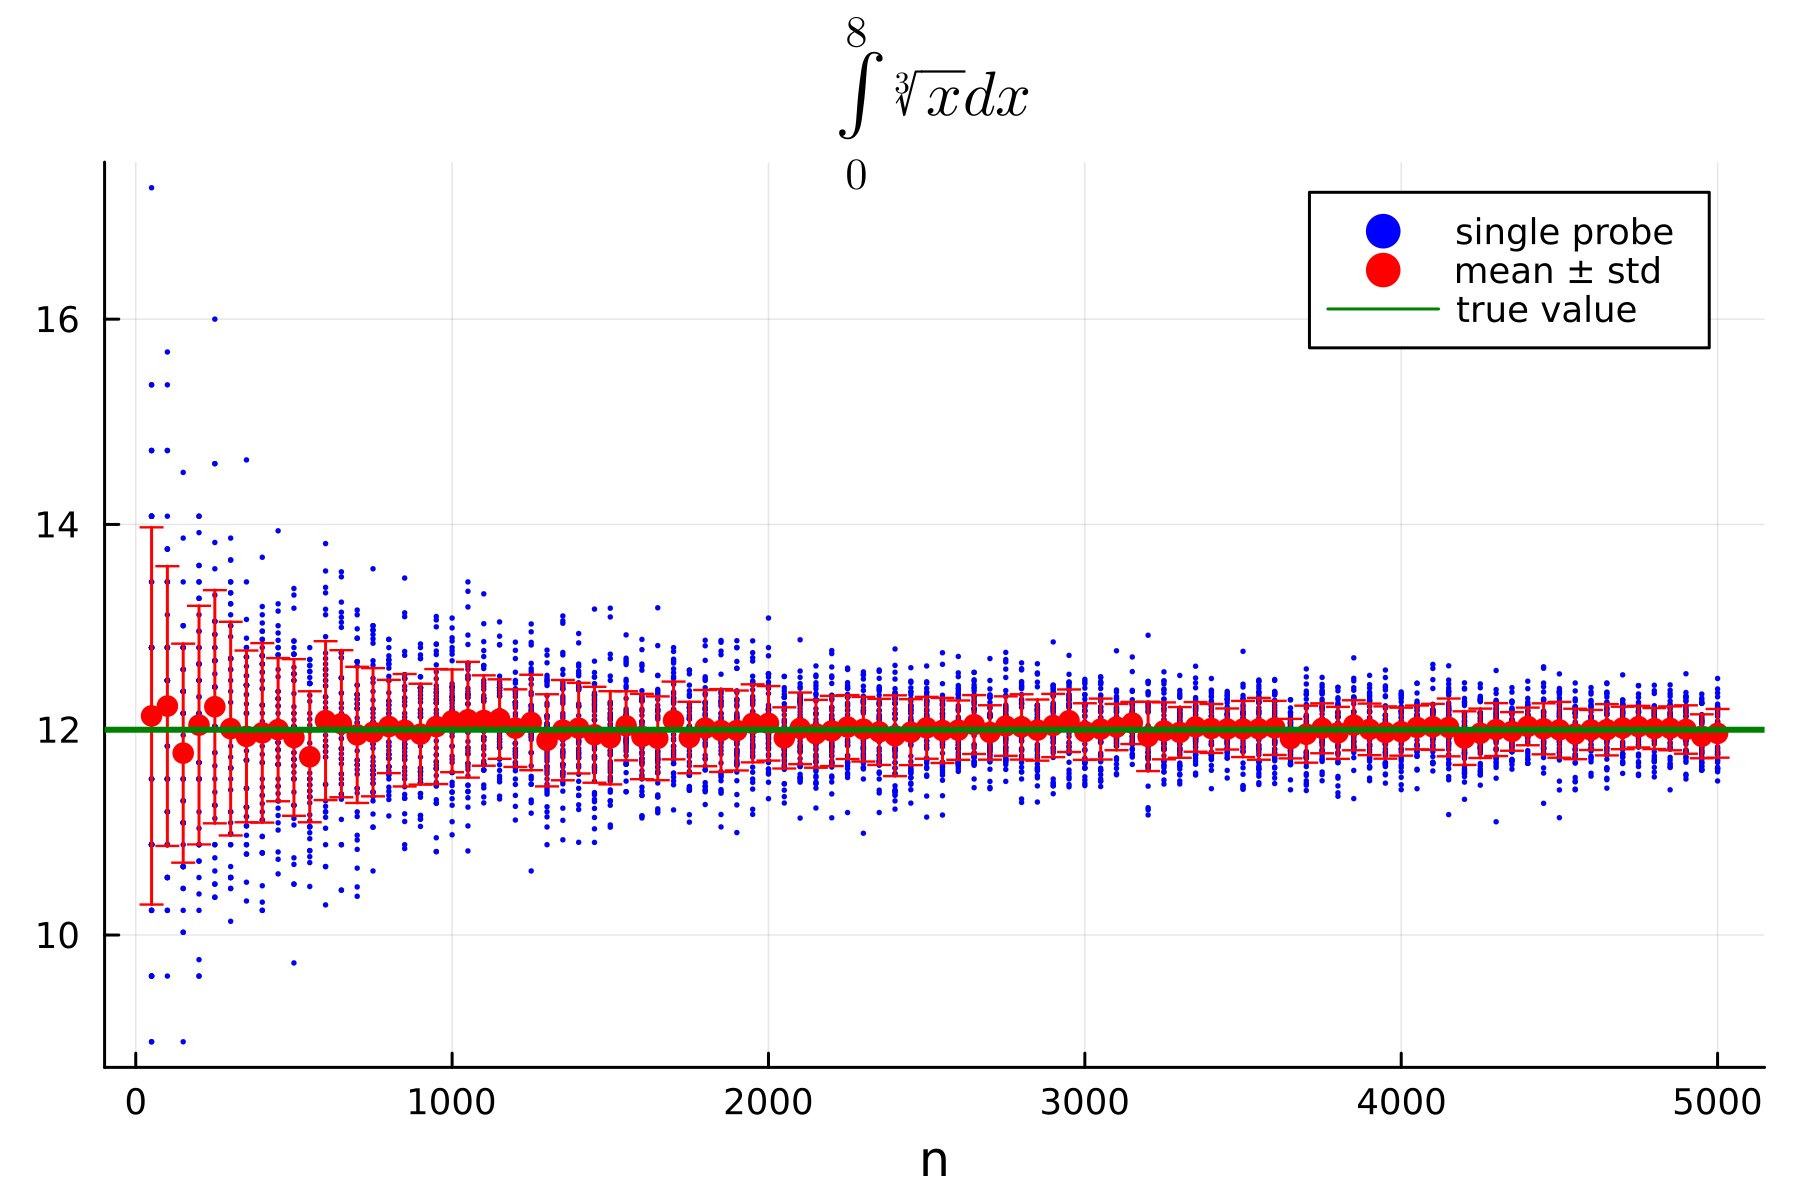
\includegraphics[width=\linewidth]{results/z1_1.png}
    \caption{Wyniki eksperymentów dla całki $\int_0^8 \sqrt[3]{x} dx$. Dla $n \in {50, 100, \dots, 5000}$, dla każdego $n$ wykonano $k=50$ niezależnych powtórzeń algorytmu. Niebieski - wynik pojedynczej aproksymacji, czerwony - średnia z $k$ powtórzeń wraz z odchyleniem standardowym jako słupkiem błędu, zielony - wartość dokładna całki.}
\end{figure}

\begin{figure}[!h]
    \centering
    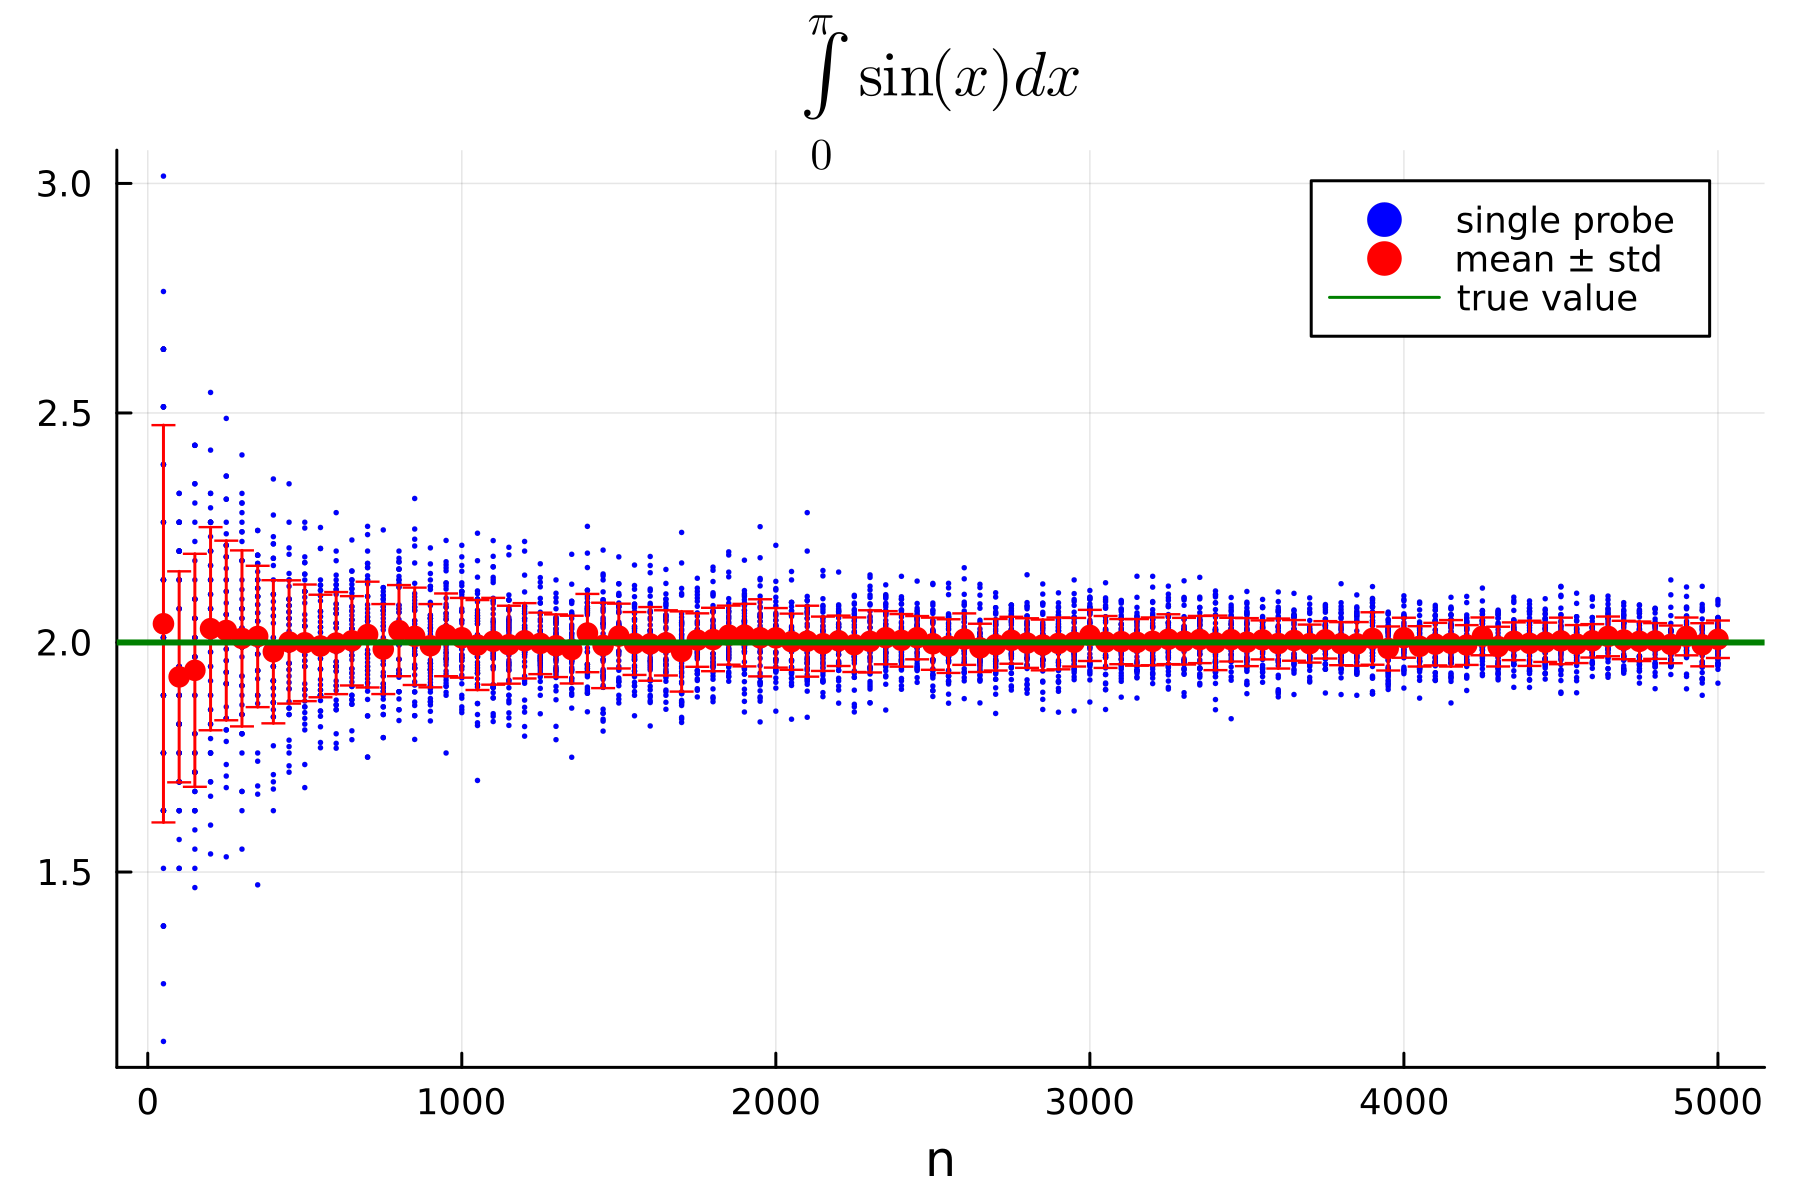
\includegraphics[width=\linewidth]{results/z1_2.png}
    \caption{Wyniki eksperymentów dla całki $\int_0^{\pi} \sin(x) dx$. Dla $n \in {50, 100, \dots, 5000}$, dla każdego $n$ wykonano $k=50$ niezależnych powtórzeń algorytmu.}
\end{figure}

\begin{figure}[!h]
    \centering
    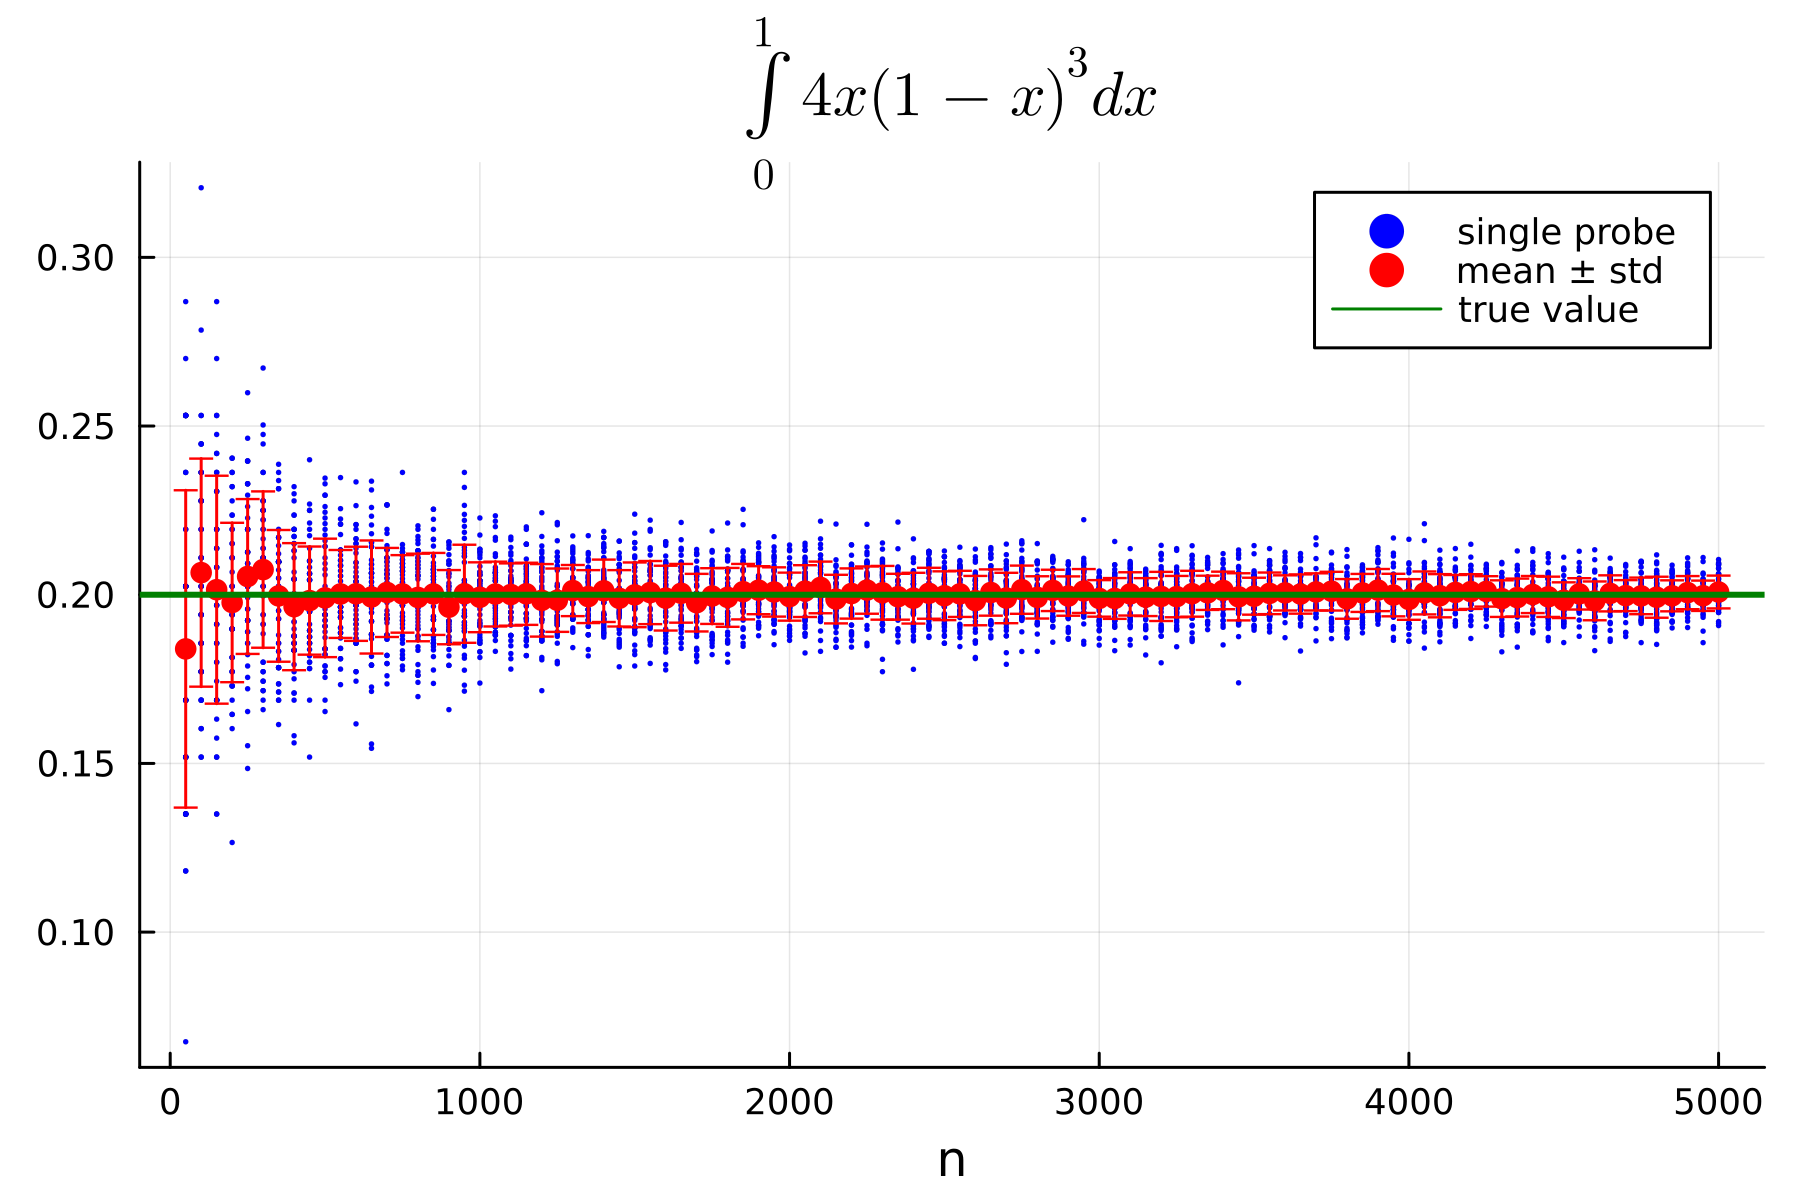
\includegraphics[width=\linewidth]{results/z1_3.png}
    \caption{Wyniki eksperymentów dla całki $\int_0^1 4x(1-x)^3 dx$. Dla $n \in {50, 100, \dots, 5000}$, dla każdego $n$ wykonano $k=50$ niezależnych powtórzeń algorytmu.}
\end{figure}



\section{Aproksymacja liczby $\pi$}

\begin{figure}[!htbp]
    \centering
    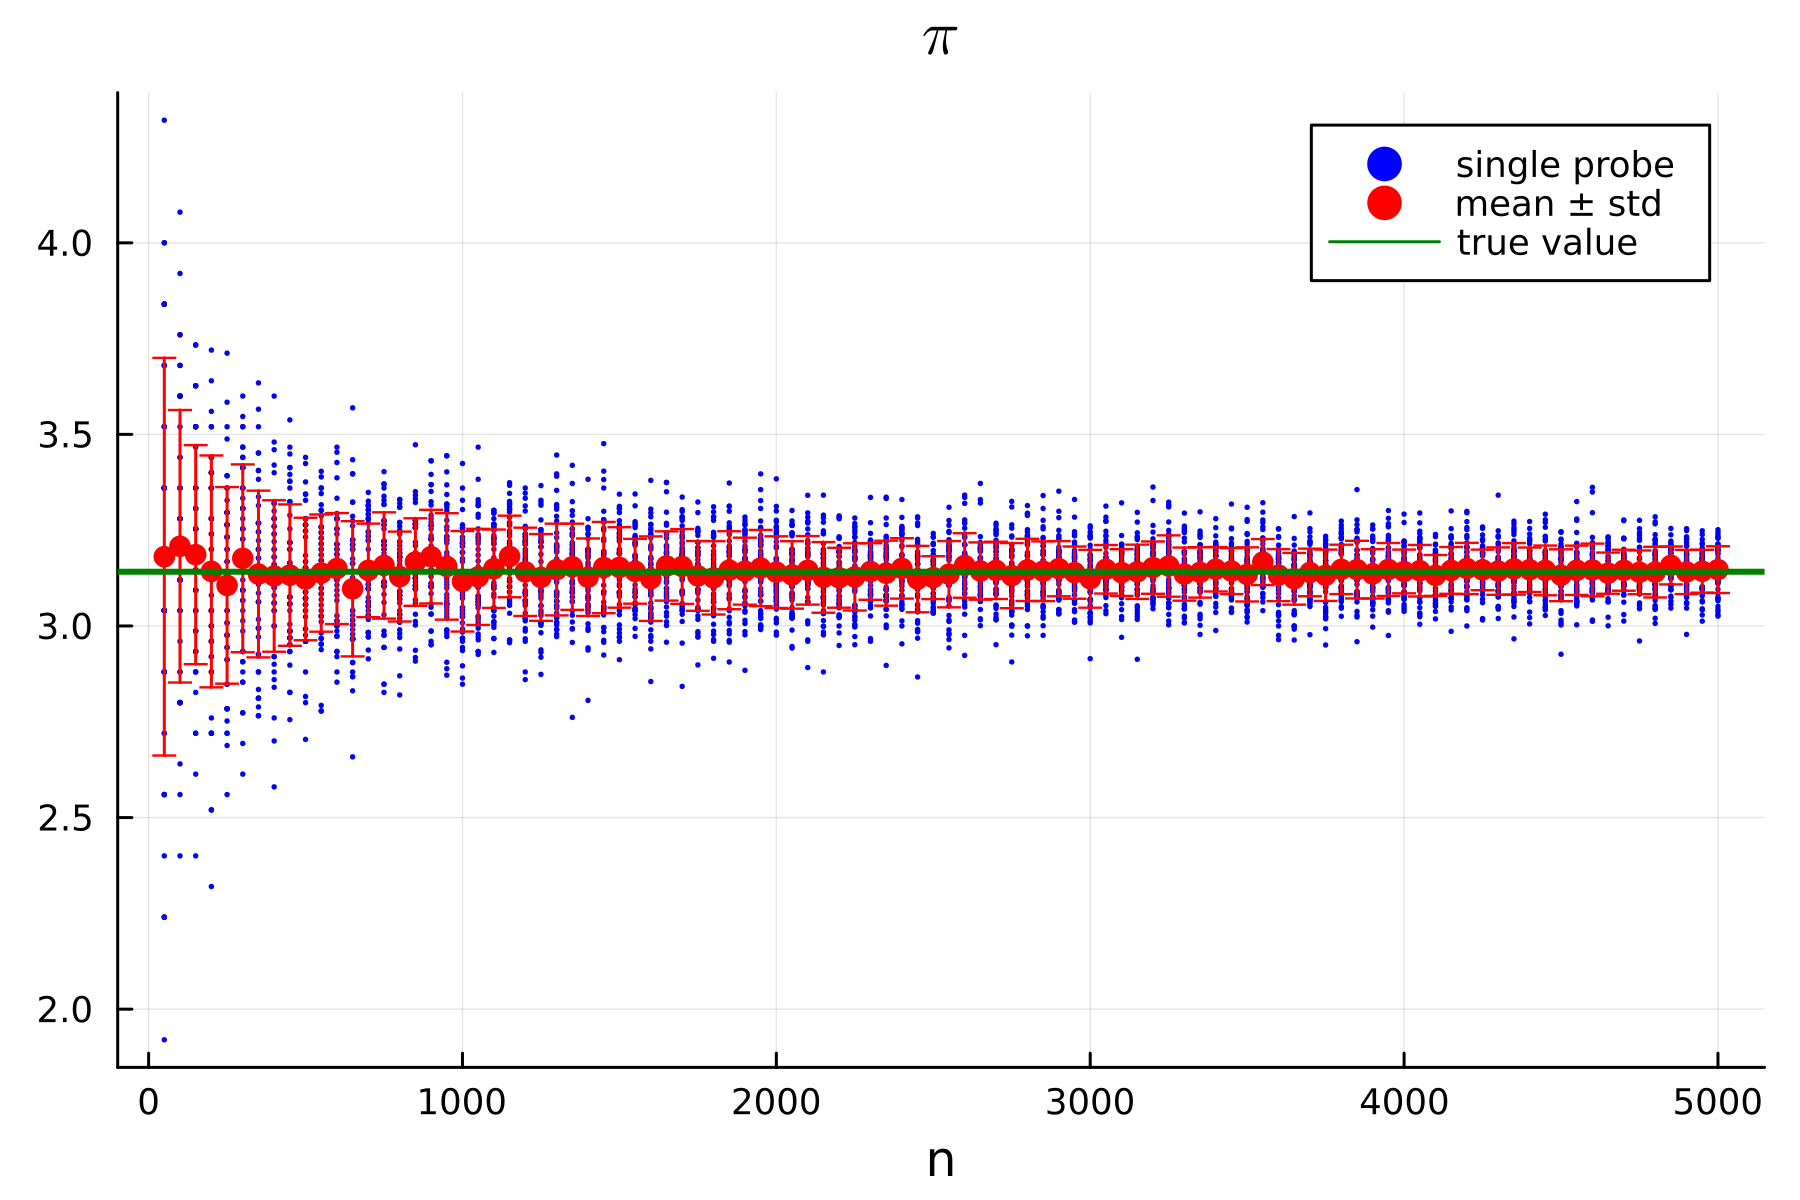
\includegraphics[width=\linewidth]{results/z1_4.png}
    \caption{Wyniki eksperymentów dla wyznaczania aproksymacji liczby $\pi$. Liczono w tym celu całkę $\int_{-1}^{1} 2\sqrt{1-x^2} dx$, której wartość dokładna wynosi $\pi$. Dla $n \in {50, 100, \dots, 5000}$, dla każdego $n$ wykonano $k=50$ niezależnych powtórzeń algorytmu.}
\end{figure}

\section{Wnioski}
Jak widać na powyższych wykresach im więcej $n$ punktów wylosowano, tym dokładniejsze wyniki uzyskano. Czyli gdy $n\rightarrow \infty$, to wartość całki aproksymowanej dąży do wartości dokładnej, a odchylenie standardowe niezależnych powtórzeń algorytmu dąży do 0.

Eksperyment wykonano w języku Julia 1.7.2.
Wartości dokładne całek zostały obliczone za pomocą programu WolframAlpha.

\end{document}
